% Options for packages loaded elsewhere
\PassOptionsToPackage{unicode}{hyperref}
\PassOptionsToPackage{hyphens}{url}
\PassOptionsToPackage{dvipsnames,svgnames,x11names}{xcolor}
\documentclass[
]{article}
\usepackage{xcolor}
\usepackage[margin=22mm]{geometry}
\usepackage{amsmath,amssymb}
\setcounter{secnumdepth}{-\maxdimen} % remove section numbering
\usepackage{iftex}
\ifPDFTeX
  \usepackage[T1]{fontenc}
  \usepackage[utf8]{inputenc}
  \usepackage{textcomp} % provide euro and other symbols
\else % if luatex or xetex
  \usepackage{unicode-math} % this also loads fontspec
  \defaultfontfeatures{Scale=MatchLowercase}
  \defaultfontfeatures[\rmfamily]{Ligatures=TeX,Scale=1}
\fi
\usepackage{lmodern}
\ifPDFTeX\else
  % xetex/luatex font selection
\fi
% Use upquote if available, for straight quotes in verbatim environments
\IfFileExists{upquote.sty}{\usepackage{upquote}}{}
\IfFileExists{microtype.sty}{% use microtype if available
  \usepackage[]{microtype}
  \UseMicrotypeSet[protrusion]{basicmath} % disable protrusion for tt fonts
}{}
\makeatletter
\@ifundefined{KOMAClassName}{% if non-KOMA class
  \IfFileExists{parskip.sty}{%
    \usepackage{parskip}
  }{% else
    \setlength{\parindent}{0pt}
    \setlength{\parskip}{6pt plus 2pt minus 1pt}}
}{% if KOMA class
  \KOMAoptions{parskip=half}}
\makeatother
\usepackage{longtable,booktabs,array}
\newcounter{none} % for unnumbered tables
\usepackage{calc} % for calculating minipage widths
% Correct order of tables after \paragraph or \subparagraph
\usepackage{etoolbox}
\makeatletter
\patchcmd\longtable{\par}{\if@noskipsec\mbox{}\fi\par}{}{}
\makeatother
% Allow footnotes in longtable head/foot
\IfFileExists{footnotehyper.sty}{\usepackage{footnotehyper}}{\usepackage{footnote}}
\makesavenoteenv{longtable}
\usepackage{graphicx}
\makeatletter
\newsavebox\pandoc@box
\newcommand*\pandocbounded[1]{% scales image to fit in text height/width
  \sbox\pandoc@box{#1}%
  \Gscale@div\@tempa{\textheight}{\dimexpr\ht\pandoc@box+\dp\pandoc@box\relax}%
  \Gscale@div\@tempb{\linewidth}{\wd\pandoc@box}%
  \ifdim\@tempb\p@<\@tempa\p@\let\@tempa\@tempb\fi% select the smaller of both
  \ifdim\@tempa\p@<\p@\scalebox{\@tempa}{\usebox\pandoc@box}%
  \else\usebox{\pandoc@box}%
  \fi%
}
% Set default figure placement to htbp
\def\fps@figure{htbp}
\makeatother
\setlength{\emergencystretch}{3em} % prevent overfull lines
\providecommand{\tightlist}{%
  \setlength{\itemsep}{0pt}\setlength{\parskip}{0pt}}
\usepackage{bookmark}
\IfFileExists{xurl.sty}{\usepackage{xurl}}{} % add URL line breaks if available
\urlstyle{same}
\hypersetup{
  colorlinks=true,
  linkcolor={Maroon},
  filecolor={Maroon},
  citecolor={Blue},
  urlcolor={Blue},
  pdfcreator={LaTeX via pandoc}}

\author{}
\date{}

\begin{document}

\section{Paper 13: Position Had Never Been Read --- Sign Sectors,
Duality Theorems, the Readout Hierarchy, and the Derived
Clock}\label{paper-13-position-had-never-been-read-sign-sectors-duality-theorems-the-readout-hierarchy-and-the-derived-clock}

\textbf{Author}: Noriaki Kihara \textbf{Date}: June 12, 2026
\textbf{Version}: v1.0 (final; v0.2 incorporated the 14 points of the
first review {[}major revision{]}, v1.0 the points R1--R5 of the second
review {[}accept with minor conditions{]}) \textbf{DOI (this version)}:
10.5281/zenodo.20665634 / \textbf{Concept DOI}: 10.5281/zenodo.20665633
\textbf{License}: CC BY 4.0 \textbf{Series}: Dual Geometry of Wavelength
Space and Frequency Space (Paper 13, sequel to Papers 1--12)

\begin{center}\rule{0.5\linewidth}{0.5pt}\end{center}

\subsection{Abstract}\label{abstract}

``Can discrete states be mapped back and forth to position and time?''
--- we answer the oldest question posed to this series' system (three
axioms: νλ=1, zero point ½, one asymmetric bit, plus configuration
reading and the record principle) with \textbf{exactly zero additions}
to the axiom inventory. Main results: (1) \textbf{Position is not a new
degree of freedom --- it was the unread part of the dictionary.}
Discrete position = the sign sector of the wave (quarter-period offsets:
cos→sin→−cos→−sin), which is merely a change in how the data already
present in the dictionary of Paper 5 is read out --- the addition to the
state space is exactly zero (Theorem 1). (2) \textbf{Space is derived}:
position space = the Pontryagin dual \(T^4\) (character group) of the
conserved-quantity lattice (charge-like) \(\mathbb{Z}^4\), and the three
symmetries --- translation, rotation, inversion --- are \textbf{theorems
of duality}, not assumptions (Definition 2, Theorems 2a--2b). No
substantial background spacetime is assumed --- position space is a
chart on relational data (line coefficients). (3) \textbf{The readout
has three strata}: the scalar data of intensity fringes (spacings)
collapse the 21 relation classes to only 11, line-position data to 13,
while \textbf{branch channels (complex line coefficients) separate all
21 orbits completely} (Theorem 3; exhaustive counts, 11 ⊂ 13 ⊂ 21) ---
the quantitative demonstration that ``position had never been read,''
locating exactly which information is lost in intensity-only readings.
(4) \textbf{The quarter-displacement theorem}: a fragment's
quarter-lattice displacement is read exactly from branch-channel phase
classes (Z₄), with the general component rule \(m\bmod4\) (Theorem 4)
--- continuous position is the hierarchical completion of these quarter
digits (the explicit map is Paper 15, to be published concurrently). (5)
\textbf{Time is resolved --- but asymmetrically to position}: the
targets \(\nu_t^2\) of the clock frequency \(\nu_t=\sqrt{s}\) run over
\textbf{all odd integers} with spacing 2 --- a \textbf{proven theorem of
unlimited range via Gauss's triangular-number theorem} (Theorem 5: for
odd \(s\), \((s-1)/2\) is a sum of four triangular numbers, always
solvable by Gauss's theorem that every natural number is a sum of three
triangular numbers). The most regular spectrum possible stands as a
proven claim. The forward map is exact on all four axes, while \textbf{t
admits no independent inverse map} (Theorem 6): \(\nu_t\) is derived as
the norm of the spatial configuration, so t has no independent scale to
round. This is not a defect but the theorem form of the
all-axes-symmetric principle --- ``t merely appears to have been
selected by observation.'' t is \textbf{easier} than xyz. This paper
claims no re-derivation of standard theory. No physical identification
is made.

\begin{center}\rule{0.5\linewidth}{0.5pt}\end{center}

\subsection{1. Introduction}\label{introduction}

\subsubsection{1.1 The fifty-year
question}\label{the-fifty-year-question}

How do continuous position \(x\) and time \(t\) coexist with a discrete
state description? For the present system the question takes the form:

\begin{quote}
Can position and time be \textbf{read out} of the system's state data
(occupied cells, branches, ledger)? If so, does the readout require an
addition to the state space (a new degree of freedom)?
\end{quote}

This paper's answer: \textbf{they can be read, with zero additions.}
Position is a re-reading of the sign sectors the dictionary (Paper 5)
has carried from the start; time is a derived quantity of the conserved
norm. What was needed was neither an axiom nor an extension but a
\textbf{change of readout principle} --- hence the title.

\subsubsection{1.2 What is not claimed}\label{what-is-not-claimed}

\begin{enumerate}
\def\labelenumi{(\roman{enumi})}
\tightlist
\item
  The explicit construction of the map to continuous coordinates
  (mixed-radix expansion, readout operation, inverse map) is carried out
  in Paper 15 (concurrent publication) --- this paper is its
  \textbf{theorem-level foundation} (what can be read; what is derived).
  (ii) The choice of time direction (why some axis looks like t) and the
  status of amplitudes are Paper 14. (iii) \textbf{This paper does not
  select an aggregation rule (measure) for path amplitudes} (the measure
  line = Paper 16, concurrent publication). (iv) No physical
  identification is made.
\end{enumerate}

\subsection{2. Preliminaries (minimal
recap)}\label{preliminaries-minimal-recap}

The dictionary of Paper 5: cell \(k\in\mathbb{Z}^4\) ↔ product wave
\(\Phi_k=\prod_j\varphi_{k_j}(x_j)\), with branch \(k_j>0\) = cos and
\(k_j<0\) = sin. Configuration reading (Paper 7): the state is the set
of occupied cells = the wave itself. The record (Papers 6/12): the
hologram \(I=\Psi^2\), whose physical content is the line coefficients
(relational data). Ledger: \(s=\sum_j(|k_j|+\tfrac12)^2\) and
\(\varepsilon=(-1)^{\Sigma|k_j|}\).

\textbf{Gauge data held fixed (complete enumeration)}: the marking \(u\)
(time-read axis), the per-axis orientations \(Z_2^{4}\) (positive branch
directions), and the reference fragment (origin). The sign-sector / Z₄
readings of Theorems 1 and 4 are \textbf{gauge-relative quantities} with
respect to these (limitation 1 of §6 connects here).

\textbf{Internal terminology declaration}: ``position'' and ``time'' in
this paper are names of readout quantities internal to the system and
carry no identification with physical quantities (naming discipline:
conserved quantities carry the ``-like'' flag, e.g.~charge-like).

\subsection{3. The resolution of
position}\label{the-resolution-of-position}

\subsubsection{3.1 Theorem 1 (sign sector = discrete position; zero
additions)}\label{theorem-1-sign-sector-discrete-position-zero-additions}

\begin{quote}
\textbf{Theorem 1}: the quarter-period translation \(T_{1/4}\) of the
fundamental wave cycles the dictionary's (branch, sign) data:
\(\cos\to\sin\to-\cos\to-\sin\) (\(d\to d+1\bmod4\)). Hence \textbf{the
(branch, sign) pair of the dictionary = quarter-period offset = discrete
position}, and introducing position requires not a single new state.
\end{quote}

\textbf{Proof} (two lines): \(\cos(\theta-\pi/2)=\sin\theta\) and
\(\sin(\theta-\pi/2)=-\cos\theta\) --- the quarter translation is the
cycle of these trigonometric identities. ∎ Machine confirmation (②):
exhaustive 4/4 (Fig. 1a). The sign sectors hitherto treated as
``alternative presentations of the same state'' were position data all
along --- only the readout principle had to change.

\subsubsection{3.2 Space = the dual of the conserved-quantity lattice
(split into definition, general theorem, and consistency
theorem)}\label{space-the-dual-of-the-conserved-quantity-lattice-split-into-definition-general-theorem-and-consistency-theorem}

\textbf{Definition 2}: position space is \textbf{defined} as the
character group (Pontryagin dual)
\(T^4=\mathrm{Hom}(\mathbb{Z}^4,U(1))\) of the conserved-quantity
lattice (charge-like) \(\mathbb{Z}^4\) (the dual chart).

\begin{quote}
\textbf{Theorem 2a (general --- a matter of proof, not of
verification)}: under this definition, (i) translation symmetry = the
group structure of the character group, (ii) rotation (B₄) symmetry =
the dual action of lattice automorphisms, (iii) inversion symmetry =
complex conjugation --- all standard theorems of Pontryagin duality.
\end{quote}

\begin{quote}
\textbf{Theorem 2b (model-specific consistency)}: the physical content
of the record (line coefficients) is a function on \(\mathbb{Z}^4\), and
the sign-sector reading of Theorem 1 embeds into this dual chart as the
per-axis \(Z_4\subset U(1)\) (quarter translation = quarter rotation of
characters). Machine confirmation (②): the 4/4 cycle of Theorem 1 is
precisely the consistency check of \(Z_4\hookrightarrow U(1)\).
\end{quote}

Consequence (background independence): position space is not a
substantial container assumed in advance but the dual chart of
relational data (lattice-indexed line coefficients). Continuous position
is obtained as the hierarchical completion of quarter digits (Fig. 1b;
explicit construction in Paper 15, Theorem 2, concurrent publication).

\subsubsection{3.3 Theorem 3 (the readout hierarchy 11 ⊂ 13 ⊂
21)}\label{theorem-3-the-readout-hierarchy-11-13-21}

The relation classes (B₄×swap orbits) of all pairs of the 64 shell-9
cells (2016 pairs) number \textbf{21}. Separating power per readout
stratum (exhaustive counts; Fig. 2):

{\def\LTcaptype{none} % do not increment counter
\begin{longtable}[]{@{}
  >{\raggedright\arraybackslash}p{(\linewidth - 4\tabcolsep) * \real{0.3333}}
  >{\raggedright\arraybackslash}p{(\linewidth - 4\tabcolsep) * \real{0.3333}}
  >{\raggedright\arraybackslash}p{(\linewidth - 4\tabcolsep) * \real{0.3333}}@{}}
\toprule\noalign{}
\begin{minipage}[b]{\linewidth}\raggedright
Readout stratum
\end{minipage} & \begin{minipage}[b]{\linewidth}\raggedright
Readable data
\end{minipage} & \begin{minipage}[b]{\linewidth}\raggedright
Separated classes
\end{minipage} \\
\midrule\noalign{}
\endhead
\bottomrule\noalign{}
\endlastfoot
Scalar fringe & spacings \((|\Delta|^2,|\Sigma|^2)\), unordered &
\textbf{11} (18 even when ordered) \\
Line-position fringe & unsigned line pair \(\{[u{+}v],[u{-}v]\}\) &
\textbf{13} \\
Branch channels & complex line coefficients (cos/sin resolution) &
\textbf{21 = complete separation} \\
\end{longtable}
}

\begin{quote}
Intensity-only reading (the traditional fringe) irrecoverably loses
\textbf{10 classes' worth of distinctions at the scalar stratum (21→11;
the pair structure of these mergers is unverified) and 8 pairs at the
line-position stratum (verified to be pairs)} out of the 21 orbits.
\textbf{The only reading that recovers all information is the branch
channel} --- the quantitative form of ``position had never been read.''
All 8 merged pairs of the line-position stratum are of the type ``sum
line confused with difference line = unreadable relative sign.''
\end{quote}

\subsubsection{3.4 Theorem 4 (readability of quarter displacements ---
the component
rule)}\label{theorem-4-readability-of-quarter-displacements-the-component-rule}

\begin{quote}
\textbf{Theorem 4}: a fragment's quarter-lattice displacement shifts the
phase class (Z₄) of the line of frequency component \(m\) by
\textbf{\(m\bmod4\)} (general rule). For the fundamental (\(m=1\)) the
shift is +1; for odd components (\(m\bmod4\in\{1,3\}\)) the shift is
invertible, so the displacement is readable.
\end{quote}

``+1'' is restricted to the fundamental (per-component \(m\bmod4\) for
multi-component fragments). This is consistent with Paper 15's digit
conventions (\(d^{(0)}\), the \(\min(c,k{-}1)\) clip) as the \(m=1\)
section of the general rule. Machine confirmation (③, sampled): the two
fringe-shift tests (tripod quarter rotation, ring inversion) PASS ---
sampled, not exhaustive. This is the operational readout of discrete
position; the hierarchical extension (peeling decode) and the continuum
are Paper 15, §5.

\subsection{4. The resolution of time}\label{the-resolution-of-time}

\subsubsection{4.1 Theorem 5 (clock targets = all odd integers --- with
proof)}\label{theorem-5-clock-targets-all-odd-integers-with-proof}

\begin{quote}
\textbf{Theorem 5}: the range of the squared clock frequency
\(\nu_t^2=s=\sum_j(|k_j|+\tfrac12)^2\) is \textbf{exactly the set of all
odd integers} (spacing 2).
\end{quote}

\textbf{Proof}: (range ⊆ odds) \(s=\sum_j|k_j|(|k_j|+1)+1\), and each
\(|k_j|(|k_j|+1)\) is a product of consecutive integers, hence
\textbf{even} --- so \(s\) is always odd. (odds ⊆ range) For any odd
\(s\), \((s-1)/2=\sum_j|k_j|(|k_j|+1)/2=\sum_j T_{|k_j|}\) is a
decomposition into \textbf{four triangular numbers}, always solvable by
Gauss's triangular-number theorem (every natural number is a sum of
three triangular numbers; the 1796 ``Eureka''), adding \(T_0=0\) as the
fourth. ∎ (Identification of the proof: first review, point \#1,
claude.ai.)

Machine confirmation (②): all 100/100 odd integers ≤ 199 reached (Fig.
3a). The clock's targets are not ``sparse and irregular'' but the most
regular possible --- \textbf{as a proven claim}. The tick at each \(s\)
is \(\Delta t=1/\sqrt{s}\) (Fig. 3b) --- the same construction as the
internal time \(t=\sum1/\sqrt{s}\) of Paper 8.

\subsubsection{4.2 Theorem 6 (no independent inverse map for
t)}\label{theorem-6-no-independent-inverse-map-for-t}

\begin{quote}
\textbf{Theorem 6 (factorization of t)}: the forward map (state →
readings of four axes) exists exactly on all four axes. In the reverse
direction: \textbf{any t-value readable from the record factorizes
through a function of \(s\)} --- there exists no readout granting t a
resolution independent of \(s\). The independent rounding (inverse map,
Paper 15, D4) that each xyz axis possesses has \textbf{no counterpart}
for t.
\end{quote}

\textbf{Proof sketch (inventory audit)}: the ledger of state data is
exhausted by occupied cells (four integer axes), branches, and signs
(configuration reading, §2). The only time-involving readings are the
norm clock \(\nu_t=\sqrt{s}\) and the event count (Theorem 5; Paper 8);
every t-dependent quantity in the record is of the form ``tick count ×
rate \(1/\sqrt{s}\)'' --- both factors functions of \(s\) and the count.
No fifth ledger entry exists in the inventory that could supply a
t-scale independent of \(s\) (finite enumeration). ∎ (sketch)

The composite round-trip check of Paper 15 (500/500) is the
\textbf{confirmation of the realization} of this theorem (the
distinction between properties of a construction and theorems).

This is a signature, not a defect: \textbf{t is not a fundamental degree
of freedom}. All axes (including R and Q) are symmetric and
interchangeable; t merely appears to have been selected by observation
--- the present theorem is the exact expression, at the level of
round-trip maps, of that principle (whose gauge form --- which axis
looks like a clock --- is the marking theorem of Paper 14). Ironically,
t is \textbf{easier} than xyz precisely because there is nothing to
round.

\subsection{5. Consequence: the present state of the fifty-year
question}\label{consequence-the-present-state-of-the-fifty-year-question}

{\def\LTcaptype{none} % do not increment counter
\begin{longtable}[]{@{}
  >{\raggedright\arraybackslash}p{(\linewidth - 4\tabcolsep) * \real{0.3333}}
  >{\raggedright\arraybackslash}p{(\linewidth - 4\tabcolsep) * \real{0.3333}}
  >{\raggedright\arraybackslash}p{(\linewidth - 4\tabcolsep) * \real{0.3333}}@{}}
\toprule\noalign{}
\begin{minipage}[b]{\linewidth}\raggedright
Question
\end{minipage} & \begin{minipage}[b]{\linewidth}\raggedright
Answer
\end{minipage} & \begin{minipage}[b]{\linewidth}\raggedright
This paper
\end{minipage} \\
\midrule\noalign{}
\endhead
\bottomrule\noalign{}
\endlastfoot
Can position be read out? & Yes (branch channels) --- zero additions &
Theorems 1, 3, 4 \\
Where do space and its symmetries come from? & Theorems of the dual of
the conserved-quantity lattice (charge-like) & Definition 2, Theorems
2a--2b \\
Can time be read out? & Forward map exact; t is derived (no independent
inverse) & Theorems 5, 6 \\
Explicit map to continuous coordinates & Constructible & Paper 15 \\
Choice of time direction; amplitudes & Theorematizable & Paper 14 \\
\end{longtable}
}

\subsection{6. Honest limits}\label{honest-limits}

\begin{enumerate}
\def\labelenumi{\arabic{enumi}.}
\tightlist
\item
  ``Position'' here is the reading of a single fragment (relative to a
  reference fragment). Common time for multiple fragments
  (synchronization) belongs to the gauge-fixing mechanism of the record
  interface and is not constructed.
\item
  The counts of Theorem 3 are exhaustive at shell 9 (s=9). The
  separation counts of the readout hierarchy at general s are uncounted
  (mechanically extensible).
\item
  Convergence and error guarantees of the continuum completion are
  deferred to Paper 15, Theorem 2.
\item
  No physical identification is made.
\end{enumerate}

\subsection{Figures}\label{figures}

\begin{itemize}
\tightlist
\item
  \textbf{Figure 1} (\texttt{paper13\_fig1\_sign\_sector.png}): (a) the
  four quarter-translates of the fundamental (cos/sin/−cos/−sin) ---
  position = sign sector. (b) nested hierarchical quarter lattices
  (refinement of index 3 per level; depth 0--2 shown)
\end{itemize}

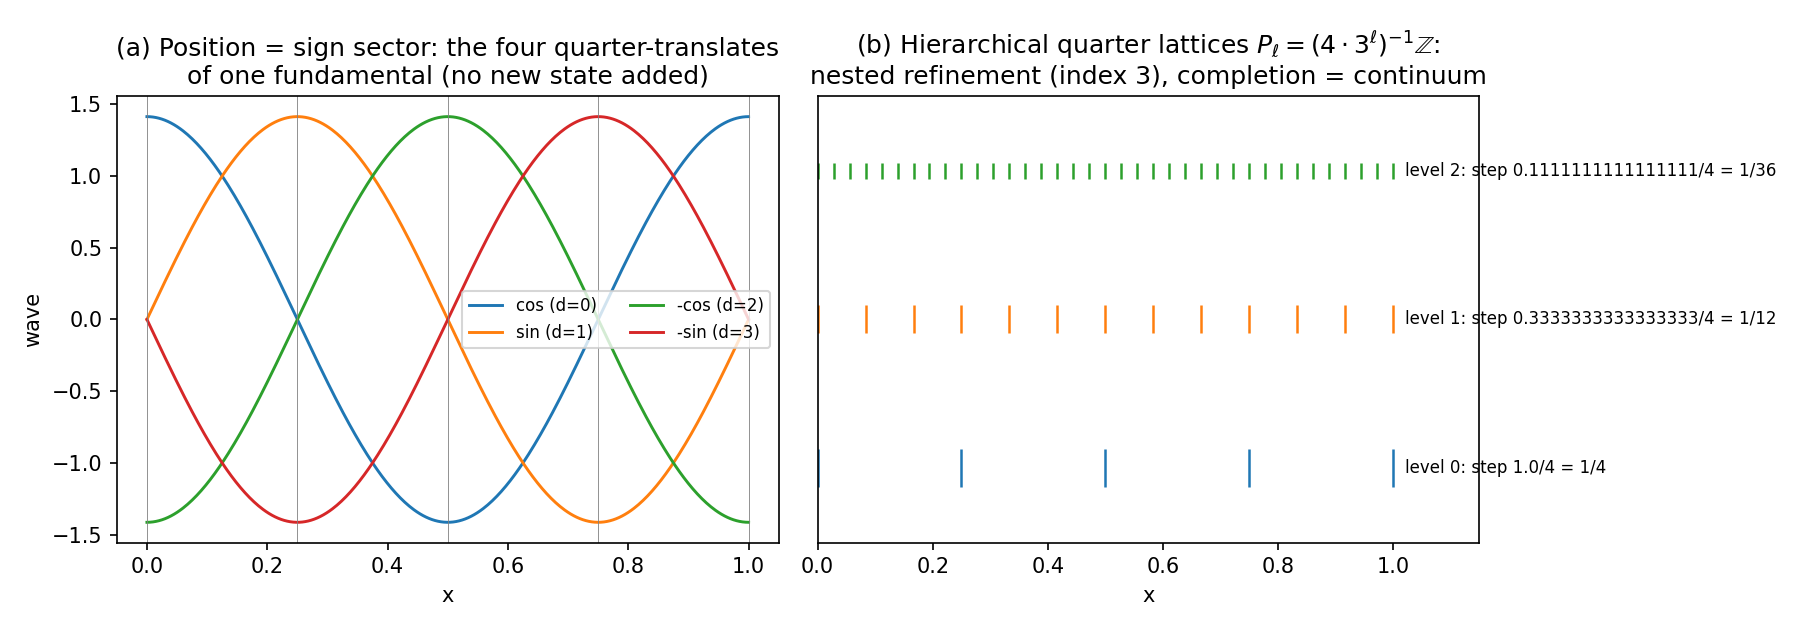
\includegraphics[width=1\linewidth,height=\textheight,keepaspectratio]{paper13_fig1_sign_sector.png}
- \textbf{Figure 2} (\texttt{paper13\_fig2\_readout\_layers.png}):
separating power of the three readout strata, 11 ⊂ 13 ⊂ 21 (exhaustive
count over all 2016 pairs)

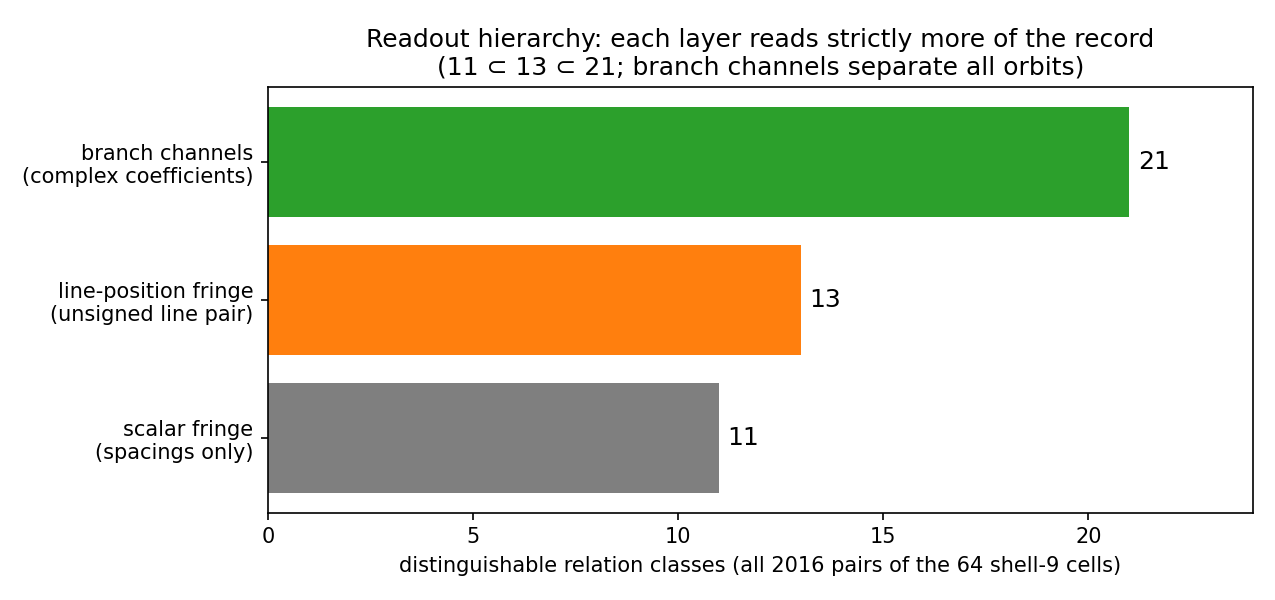
\includegraphics[width=1\linewidth,height=\textheight,keepaspectratio]{paper13_fig2_readout_layers.png}
- \textbf{Figure 3} (\texttt{paper13\_fig3\_derived\_time.png}): (a)
clock targets = all odds (100/100 below 199, spacing 2). (b) tick
\(\Delta t=1/\sqrt{s}\) --- no independent scale for t

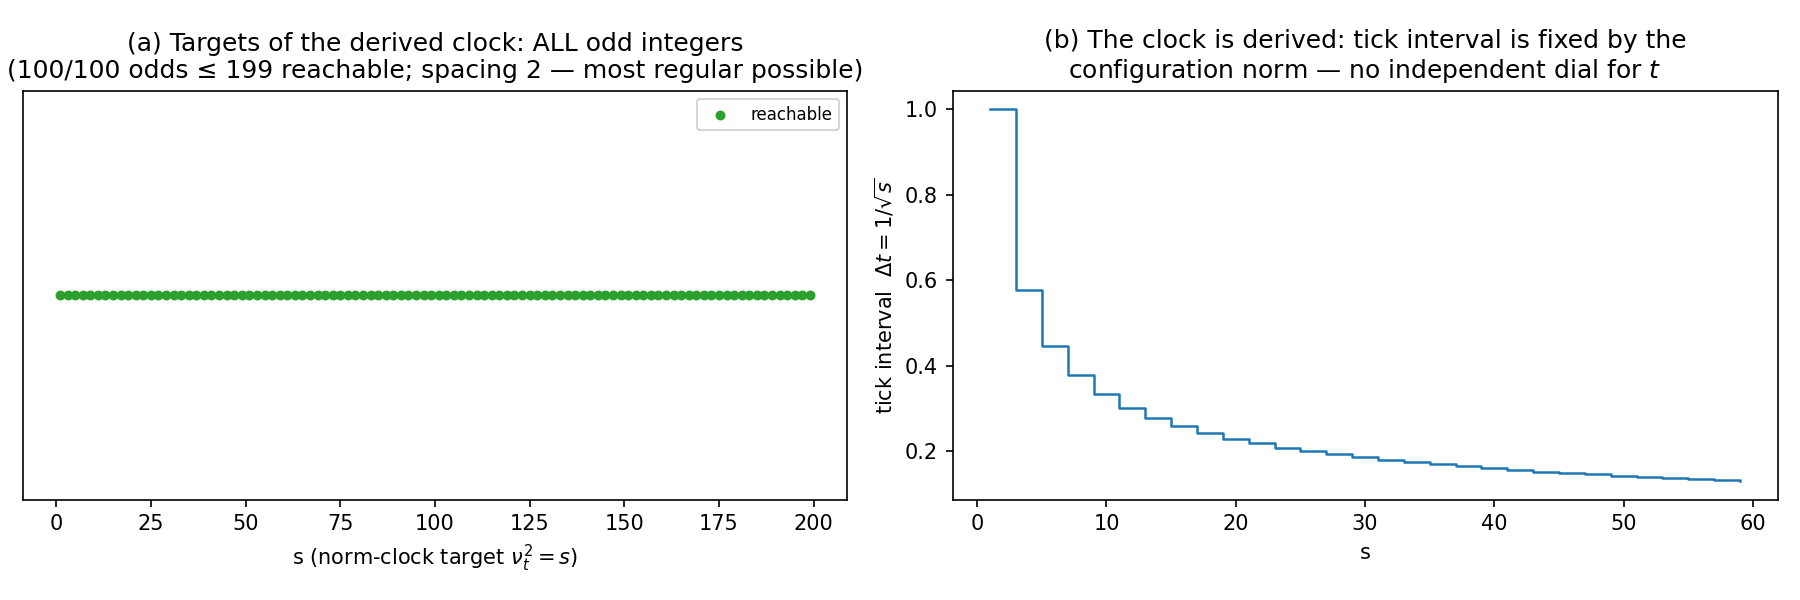
\includegraphics[width=1\linewidth,height=\textheight,keepaspectratio]{paper13_fig3_derived_time.png}

All figures are exact computations (no schematics).

\subsection{Appendix A: Verification summary (labels: ① true by
construction / ② theorem + confirmation / ③ check that could have
failed)}\label{appendix-a-verification-summary-labels-ux2460-true-by-construction-ux2461-theorem-confirmation-ux2462-check-that-could-have-failed}

{\def\LTcaptype{none} % do not increment counter
\begin{longtable}[]{@{}
  >{\raggedright\arraybackslash}p{(\linewidth - 8\tabcolsep) * \real{0.2000}}
  >{\raggedright\arraybackslash}p{(\linewidth - 8\tabcolsep) * \real{0.2000}}
  >{\raggedright\arraybackslash}p{(\linewidth - 8\tabcolsep) * \real{0.2000}}
  >{\raggedright\arraybackslash}p{(\linewidth - 8\tabcolsep) * \real{0.2000}}
  >{\raggedright\arraybackslash}p{(\linewidth - 8\tabcolsep) * \real{0.2000}}@{}}
\toprule\noalign{}
\begin{minipage}[b]{\linewidth}\raggedright
Claim
\end{minipage} & \begin{minipage}[b]{\linewidth}\raggedright
Label
\end{minipage} & \begin{minipage}[b]{\linewidth}\raggedright
Verification
\end{minipage} & \begin{minipage}[b]{\linewidth}\raggedright
Method
\end{minipage} & \begin{minipage}[b]{\linewidth}\raggedright
Script
\end{minipage} \\
\midrule\noalign{}
\endhead
\bottomrule\noalign{}
\endlastfoot
Theorem 1 (quarter translation = digit shift) & ② (proof given) & 4/4 &
exhaustive confirmation & supplement62\_projection\_formalization.py \\
Theorem 2a (duality, general) & --- (proof matter; not subject to
verification) & --- & --- & --- \\
Theorem 2b (\(Z_4\hookrightarrow U(1)\) consistency) & ② & same 4/4 as
Theorem 1 & exhaustive confirmation & same \\
Theorem 3 (11/13/21) & ③ & all 2016 pairs & \textbf{exhaustive} &
supplement79\_scale\_free\_and\_stripe\_table.py,
supplement81\_mirror\_lemma\_check.py (scalar fringe),
paper13\_14\_figures.py \\
Complete separation of 21 orbits (branch channels) & ③ & 21/21 &
exhaustive & supplement44\_branch\_channel\_verification.py \\
Theorem 4 (readability of displacements) & ③ & 2 fringe-shift tests PASS
& \textbf{sampled} & supplement44\_branch\_channel\_verification.py \\
Theorem 5 (all odds) & ② (proof by Gauss's theorem) & 100/100 odds ≤ 199
& in-range confirmation & paper13\_14\_figures.py \\
Theorem 6 (t factorization) & ② (inventory-audit sketch) & Paper 15
round trip 500/500 as realization check & cross-check &
supplement62\_inverse\_roundtrip\_test.py \\
\end{longtable}
}

\begin{center}\rule{0.5\linewidth}{0.5pt}\end{center}

\textbf{Acknowledgments / history}: verification was carried out under
the two-party independent verification protocol of Claude Code (local
machine verification) and claude.ai (independent re-computation).
Precise record of verification scope: the three-stratum counts on the
64-cell domain (11/13/21) are Claude Code verifications; claude.ai
confirmed method equivalence on the 48-cell domain (13/8) --- the
independent 64-domain recomputation is registered in claude.ai's queue.
The proof of Theorem 5 is due to the identification of Gauss's
triangular-number theorem (claude.ai, first review \#1). The prototype
of Theorem 6 is Supplement 48 (June 12, 2026). Source material:
Supplements 43, 44, 47 (branch-channel part only), 48, 79, 81 (June 12,
2026). v0.2: 14 points of the first review (major revision). v1.0:
points R1--R5 of the second review (accept with minor conditions).

No physical identification is made.

\end{document}
